\documentclass{beamer}
\usepackage{amsmath}
\usepackage{amsthm}
\usepackage{amssymb}
\usepackage[style=apa]{biblatex}
\bibliography{sources.bib}
\usepackage{hyperref}
\usepackage[shortlabels]{enumitem}
\usetheme{Boadilla}
\usepackage{tcolorbox}

\usepackage{tikz}
\usetikzlibrary{positioning, calc}

\title{Energy-based Associative Memories}
\author{Connor Hanley}

\begin{document}

\begin{frame}
    \maketitle
\end{frame}

\begin{frame}
    \frametitle{Outline of Presentation}
    \tableofcontents
\end{frame}

\section{Associative Memories}
\begin{frame}
\frametitle{Associative Memories}

\begin{definition}[Associative memory]
    An \textit{associative memory} is a $3$-tuple $\langle f, A, C \rangle$
    obeying the following properties\footnote{Following the definition from 
    \parencite{kanerva_sparse_1993}}:
    \begin{enumerate}[(i)]
        \item The \textit{address} matrix $A$ is an $N \times D$ matrix of 
        patterns we wish to learn as \textit{cues} or \textit{queries};\label{def:assoc:cond1}
        \item The \textit{content} matrix $C$ is an $N \times M$ matrix of
        patterns we wish to learn as \textit{responses}, or associate with 
        each $a_i$, $i = 1, 2, \dots, N$; and, \label{def:assoc:cond2}
        \item The \textit{recall} function 
        $f_{A, C} : \mathbb{R}^D \to \mathbb{R}^M$ maps $D$-dimensional query or 
        cue patterns $x$ to memorized $M$-dimensional patterns $y$. \label{def:assoc:cond3}
    \end{enumerate}
\end{definition}\label{def:assoc}

\end{frame}

\begin{frame}
    \begin{enumerate}[(a)]
        \item Associative memories learn to associate patterns $(x, y)$ in the 
        learning phase
        \item Typically the task is to recall $y$ based on noisy, masked, or 
        degraded forms of $x$
        \item An associative memory is said to be \textit{auto-associative} 
        if $x = y$ (therefore $A = C$)
        \item It is said to be \textit{hetero-associative} otherwise
    \end{enumerate}
\end{frame}

\section{Correlation Matrix based AMs}
\begin{frame}
\frametitle{Correlation Matrix based AMs}
\begin{enumerate}[(a)]
    \item There are many different kinds of associative memories
    \item The kind of memory that we will be focusing on here are 
    \textit{correlation matrix} based memories \parencites{nakano_associatron-model_1972,amari_learning_1972,hopfield_neural_1982,hopfield_neurons_1984,anderson_correlation_1988}
\end{enumerate}

\begin{definition}[Correlation Matrix AM]
    A \textit{correlation matrix} AM is a tuple $\langle f, A, C \rangle$
    with:
    \begin{enumerate}[(i)]
        \item Standard $N \times D$ address matrix,
        \item Standard $N \times M$ content matrix,
        \item Recall function:
        \begin{align*}
        f_{A, C} (x) &= g(W x), \\
        \text{with}~W &= C^\top A. \\
        \end{align*} \label{def:correlation:cond3}
    \end{enumerate}
\end{definition}

\end{frame}

\begin{frame}
    The function $g$ in~\autoref{def:correlation:cond3} is either:
    \begin{enumerate}[(a)]
        \item In \textcite{anderson_correlation_1988} the identity function
        $g(x) = x$
        \item In \textcites{amari_learning_1972,nakano_associatron-model_1972,hopfield_neural_1982},
        $g(x) = \text{sgn}\left\{x\right\}$, with
        $$
        \text{sgn} \left\{n\right\} = \begin{cases}
            -1,~&\text{if}~n < 0, \\
            0,~&\text{if}~n= 0, \\
            1,~&\text{if}~ n > 0.
        \end{cases}
        $$
        called the \textit{signum} function.
    \end{enumerate}
\end{frame}

\begin{frame}
\frametitle{Kohonen Network versus Amari Network}

\centering
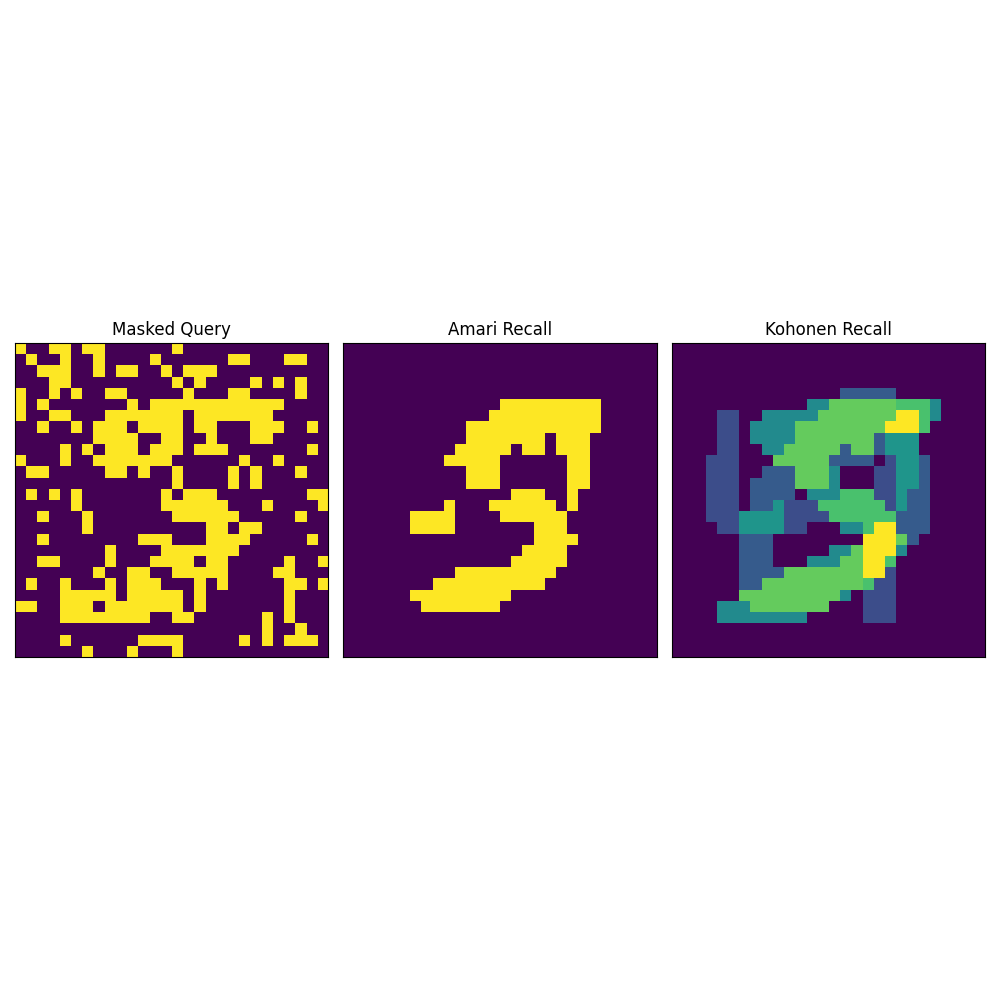
\includegraphics[width=\textwidth,scale=0.5]{amari_kohonen.png}

\end{frame}

\begin{frame}
    \centering
    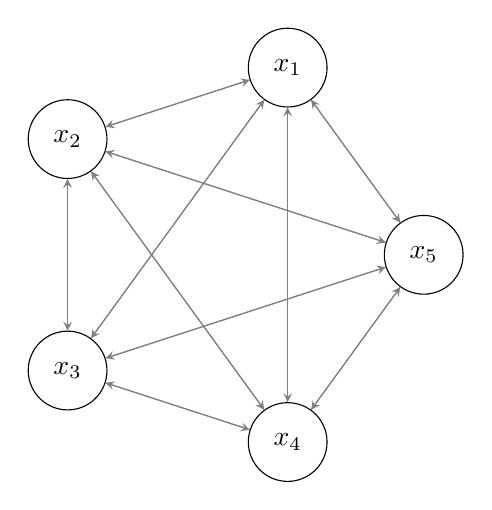
\begin{tikzpicture}[
      neuron/.style={circle, draw, minimum size=1cm, fill=white},
      connection/.style={-stealth, gray, thin}
  ]

  \newcommand{\numneurons}{5}

  \foreach \i in {1,...,\numneurons} {
      \node[neuron] (n\i) at (360/\numneurons*\i:2.5cm) {\(x_{\i}\)};
  }

  \foreach \i in {1,...,\numneurons} {
    \foreach \j in {1,...,\numneurons} {
      \ifnum\i=\j\else
        \path (n\i) -- (n\j) coordinate[midway] (mid);
        \draw[connection] (n\i) -- (n\j) 
          node[pos=0.7, above, sloped, font=\tiny] {};
      \fi
    }
  }
  \end{tikzpicture}
  Where each connection is $w_{ij} = w_{ji}$.
\end{frame}

\section{Hebbian Learning}
\begin{frame}
\frametitle{Hebbian Update Rules}
\begin{definition}[Hebbian update-rule; Hebbian learning]
    Let $x_n$, $n = 1, 2, \dots, L$ be a \textit{layer} of computational
    units, up to $L$ layers. Let the weights $W_{ij}$ be a matrix 
    representing the weights of full connections between layers $x_i$ and
    $x_j$. Then, we say that a weight update rule is \textit{Hebbian} iff
    $$
    \Delta W_{ij} = f(x_i, x_j).
    $$
\end{definition}

\begin{example}[Activity Product Rule]
    The simplest form of Hebbian learning is the following update rule\footnote{\parencite{haykin_neural_2009}}:
    $$
    \Delta W_{ij} = \eta x_j x_i^\top,
    $$
    where $\eta$ is the \textit{learning rate}.
\end{example}
\end{frame}

\begin{frame}
\frametitle{Correlation Matrix Memories are Hebbian}

We can formulate Correlation Matrix AM learning of patterns as Hebbian.
Let $\xi_\mu$, $\mu = 1, 2, \dots, N$ be the $N$ patterns of $D$ dimension
that we want the system to memorize. For each time step, suppose we present
a new pattern $\xi_{t=\mu}$:
\begin{align*}
W^{(0)} &\gets [0]_{D \times D}, \\
W^{(t+1)} &\gets W^{(t)} + \eta \xi_i \xi_i^\top.
\end{align*}
Formulated as a difference,
$$
\Delta W = \eta \xi_i \xi_i^\top.
$$
At time $t = \mu$, this is equivalent to the matrix:
$$
W = \sum^N_{\mu=1} \xi_\mu \xi_\mu^\top = \Xi^\top \Xi,
$$
with $N \times D$ pattern matrix $\Xi = [\xi_1, \xi_2, \dots, \xi_N]$.
\end{frame}

\section{Energy Minimization, Energy Descent}
\begin{frame}
\frametitle{Energy and Correlation Matrix (Hopfield!)}
Correlation Matrix AMs can be understood as performing \textit{energy minimization}.
In the same way that we can specify the \textit{weight dynamics} with the update 
rule, we can also specify the \textit{neural dynamics} of the Hopfield network;
i.e., asynchronous update rules.
\begin{definition}[Hopfield energy]
    Let $\Xi = [\xi_1, \xi_2, \dots, \xi_N]$ be the $N \times D$ pattern matrix.
    Let $W = \Xi^T \Xi$. Let $\sigma$ be a $D$-dimensional query vector. The
    \textit{energy} \parencites{krotov_dense_2016,hopfield_neurons_1984} of the 
    AM given the query vector $\sigma$ is the 
    \textit{dot product correlations} between the weights and the query vector:
    $$
    E_\text{Hopfield} = - \frac{1}{2} \sum^N_{i,j} W_{ij} \sigma_i \sigma_j = 
    - \frac{1}{2} \sum^N_{\mu=1} \left( \sum^D_{i=1} \Xi_{\mu i} \sigma_i \right)^2.
    $$
\end{definition}
\end{frame}

\begin{frame}
    \begin{tcolorbox}[colback=blue!5, colframe=blue!40, title=Energy intuition]
        The \textbf{energy} of a Hopfield network is the \textit{weighted} dot 
        product between each computational unit and every other. Low energy
        means there is \textit{high} correlation between the value of each 
        comptuational unit and the others. High energy means that there is 
        \textit{low} correlation between each computational unit and every other.
    \end{tcolorbox}
\end{frame}

\begin{frame}
\frametitle{Asynchronous update rule}
    In the energy-based framework, the AM is updated \textit{asynchronously}.
    At each time step $t$, we pick a random neuron and flip its value. If this
    value \textit{lowers} the energy, then we keep the flip. Otherwise, we 
    pick another random value.

    \begin{definition}[Asynchronous Hopfield update rule]
        \begin{align*}
        \sigma^{(t+1)}_i &= \text{argmin}_{b \in \{-1, 1\}}[E_\text{Hopfield}(\sigma'_i)]
        \end{align*}
        with $\sigma' = \sigma^{(t)}$, but with the $i$'th element set to $b$.
    \end{definition}
\end{frame}

\begin{frame}
    \begin{fact}[One-step rule relation to asynchronous rule]
        The asynchronous rule defined above relates to the single-pass update
        rule as you can derive the single-pass rule from the difference of 
        the energies of the query buffer with the $i$'th unit flipped and unflipped.
        \parencite{krotov_modern_2025,mimura_dynamical_2025}.
    \end{fact}
\end{frame}

\begin{frame}
\frametitle{Energy Dynamics}

    \begin{figure}
        \centering
        \includegraphics[scale=0.15]{hopfield.png}
        \caption{``Neurodynamics'' of the Hopfield energy function. From \textcite{haykin_neural_2009},
        originally from \textcite{hopfield_neurons_1984}.}
    \end{figure}

\end{frame}

\begin{frame}
\frametitle{Energy-based Recall (Demonstration)}

\centering
\begin{figure}
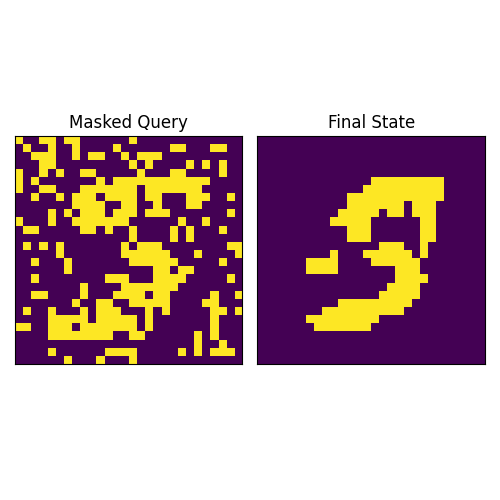
\includegraphics[width=\textwidth, height=\textheight]{hopfield_recall_states.png}
\end{figure}

\end{frame}

\begin{frame}
\centering
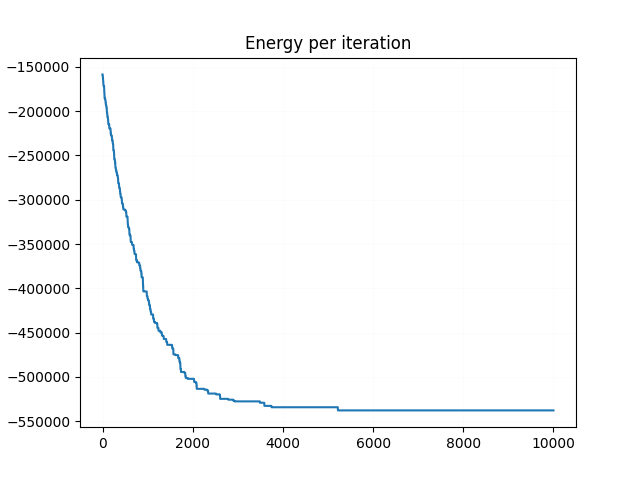
\includegraphics[width=\textwidth, height=\textheight]{hopfield_recall_energy.png}
\end{frame}

\section{Dense Associative Memories}

\begin{frame}
\frametitle{Increasing storage capacity with Dense Associative Memories}
\begin{itemize}
\item Convergent investigation into Dense Associative Memory-like models began
soon after \textcite{hopfield_neural_1982} with 
\textcites{hintzman_minerva_1984}. Tensor-based energy functions and weights
with \textcites{chen_high_1986,psaltis_nonlinear_1986} (see also, \textcite{kelly_memory_2017}).

\item Hopfield networks famously have a capacity for $\sim 0.14D$ memories, where
$D$ is the dimension of the patterns to store; note that this is can be even
further diminished by correlated patterns, introducing ``cross-talk'' 
(note even in \textcite{anderson_correlation_1988})

\end{itemize}
\end{frame}

\begin{frame}
\frametitle{Generalized Energy Function}

\begin{definition}[Generalized Energy Function]
    Consider the following abstraction of $E_\text{Hopfield}$:
    $$
    E_{F_n} = - \sum^N_{\mu=1} F \left(\sum^D_{i=1} \xi_{\mu i} \sigma_i \right)
    $$
    We call $F_n$ the \textit{Lagrangian} function \parencite{krotov_hierarchical_2021}.
    $F_n$ is of the form $\frac{1}{n} (x)^n$.
\end{definition}
\end{frame}

\begin{frame}
We can also get an update rule from this:
\begin{definition}[Generalized Update Function]
    For energy function with Lagrangian $F_n$, $E_{F_n}$, the single-pass update
    function is \parencites{krotov_dense_2016,krotov_hierarchical_2021,demircigil_model_2017}:
    $$
    \sigma^{(t+1)} = \text{sgn} \left\{ \sum^N_{\mu=1} \xi_{\mu i} F_n' \left( \sum^D_{j \neq i} \xi_{\mu j} \sigma_j\right) \right\},
    $$
    equivalently,
    $$
    \sigma^{(t+1)} = \text{sgn} \left\{ \Xi^T F' \left( \Xi \sigma \right)\right\}
    $$
\end{definition}
    
\end{frame}

\begin{frame}
    \begin{example}[Classical Hopfield]
        The above definition gets us the classical Hopfield energy function immediately,
        with energy,
        $$
        E_\text{Hopfield} = E_{F_2} = - \frac{1}{2} \sum^N_{\mu=1} \left( \sum^D_{i=1} \xi_{\mu i} \sigma_i  \right)^2;
        $$
        and update:
        $$
        \sigma^{(t+1)} = \text{sgn}\left\{ \Xi^T \Xi \sigma^{(t)} \right\}.
        $$
    \end{example}
\end{frame}

\begin{frame}
    \begin{example}[\textsf{Minerva2}]
        We can also get \textsf{Minerva2} (and more generally, every \textsf{Minerva} model)
        \parencites{hintzman_minerva_1984,kelly_memory_2017}:
        \footnote{To see further corresp. with Memory Tesseract, note that $F_4$ gives $4$-way interaction
        term in the weights.}
        $$
        E_\mathsf{Minerva2} = E_{F_4} = - \frac{1}{4} \sum^N_{\mu =1} \left( \sum^D_{i=1} \xi_{\mu i} \sigma_i \right)^4;
        $$
        and update rule:
        $$
        \sigma^{(t+1)} = \text{sgn} \left\{ \Xi^T \left( \Xi \sigma^{(t)} \right)^3 \right\}.
        $$
    \end{example}
\end{frame}

\section{Capacity}
\begin{frame}
\frametitle{Capacity}

\begin{itemize}
    \item There are many ways to characterize the capacity of an AM; note that since
    it is totally defined, we won't get ``out-of-bounds'' memory access or null-pointers

    \item The trade off is we get a ``crap-in-crap-out'' phenomenon: if the memory
    is filled with too many items, we enter into \textit{spurious} energy states

    \item Dense Associative Memory theory gives us the following relation:
\end{itemize}
\begin{theorem}[Capacity scaling laws]
    We say that $N^\text{max}$ is the number of patterns the AM can store (
        literature uses $K$, see \textcite{krotov_dense_2016}
    ). With Lagrangian function $F_n$, $N^\text{max}$ scales exponentially with
    $n$:
    $$
    N^\text{max} \propto N^{n-1}.
    $$
\end{theorem}
Proof is ommitted. See \textcites{krotov_dense_2016,demircigil_model_2017}.

\end{frame}

\begin{frame}
    \begin{lemma}[Capacity of \textsf{Minerva2}]
        We immediately get from the above that the capacity of \textsf{Minerva2}
        is:
        $$
        N^\text{max} \propto N^3.
        $$ 
    \end{lemma}
\end{frame}

\begin{frame}
\frametitle{Modern Hopfield Networks}

So far we have been dealing with bipolar values $x \in \{-1, 1\}$: but this
perspective can be expanded to real values. Namely, Modern Hopfield Networks
\parencite{ramsauer_hopfield_2021} which are equivalent to Multi-head Attention
in Transformers \parencite{vaswani_attention_2023}.

\begin{definition}[Modern Hopfield]
    Energy of multi-head attention relies on the Lagrangian function \textit{logsumexp},
    defined as:
    $$
    \text{lse} (\beta, x) = \frac{1}{\beta} \log \left( \sum^D_{i=1} \exp (\beta x_i)\right).
    $$
    This gives us an update rule
    $$
    \sigma^{(t+1)} = \Xi^T \text{softmax} \left(\beta \Xi \sigma^{(t)}\right).
    $$
\end{definition}
\end{frame}

\begin{frame}
\frametitle{If you're interested in this}

\begin{enumerate}[(a)]
    \item This was just the summary of general results
    \item There is a new framework for architecture agnostic energy-descent
    networks, called HAMUX \parencite{krotov_hierarchical_2021}
    \item HAMUX gets you compositional energy functions, and an energy-descent
    rule which is in terms of all of the different parts of the network
    \item I'm not too familiar with it, so I didn't talk about it here.
\end{enumerate}

\end{frame}

\section{Problem: Hebbian Dense Associative Memory?}
\begin{frame}
\frametitle{DAM Not Hebbian}
    \begin{enumerate}[(a)]
        \item Closing remarks: DAM is not Hebbian. This is because the weight update
        rule requires multiple interaction terms, again see \textcite{kelly_memory_2017}.

        \item Training usually proceeds using conventional methods: backpropagation or 
        even predictive coding \parencites{millidge_predictive_2022,salvatori_associative_2021}

        \item can we make a Hebbian network which 
        has similar scaling laws and capacity as DAMs?
    \end{enumerate}
\end{frame}

\begin{frame}[allowframebreaks]
    \frametitle{Bibliography}
    \printbibliography
\end{frame}


\end{document}